%----------------------------------------------------------------------------------------
%	APPENDIX
%----------------------------------------------------------------------------------------

\section{Additional figures}
\label{apx:AdditionalFigures}

\begin{figure}[h]
	\centering
	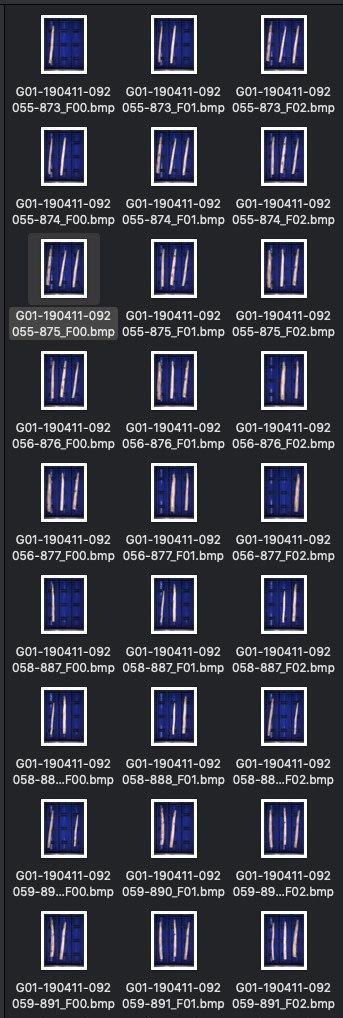
\includegraphics[scale=0.4]{Figures/appendix/original_files_naming_conventions.png}
	\decoRule
	\caption[File Overview Example of Original Image Data]{\textbf{File Overview Example of Original Image Data}~~~View of the data files after data collection. The original file names can be seen. The images belonging to one asparagus are marked with F00, F01, and F02 respectively.}
	\label{fig:Original_Data_Overview}
\end{figure}

\subsection{Single-label CNN}
\label{sec:AdditionalSingleLabelCNN}

\begin{figure}[!htb]
	\centering
	\begin{subfigure}{0.3\textwidth}
		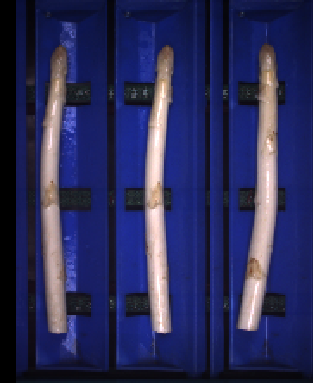
\includegraphics[width=0.9\linewidth]{Figures/appendix/violet_falsenegative_01.png}
		\vspace{-5pt}
		\caption{False Negative}
	\end{subfigure}
	\begin{subfigure}{0.3\textwidth}
		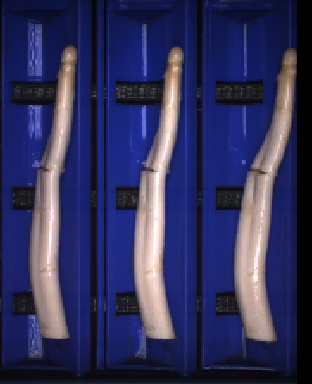
\includegraphics[width=0.9\linewidth]{Figures/appendix/violet_falsenegative_02.png}
		\vspace{-5pt}
		\caption{False Negative}
	\end{subfigure}
	\begin{subfigure}{0.3\textwidth}
		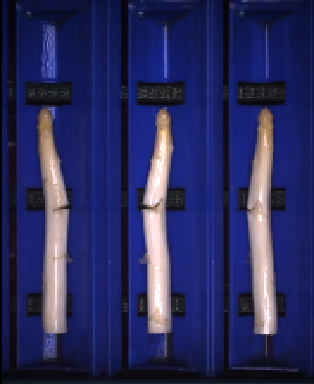
\includegraphics[width=0.9\linewidth]{Figures/appendix/violet_falsenegative_03.png}
		\vspace{-5pt}
		\caption{False Negative}
	\end{subfigure}

	\begin{subfigure}{0.3\textwidth}
		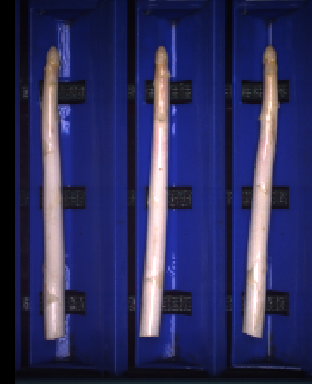
\includegraphics[width=0.9\linewidth]{Figures/appendix/violet_falsepositive_01.png}
		\vspace{-5pt}
		\caption{False Positive}
	\end{subfigure}
	\begin{subfigure}{0.3\textwidth}
		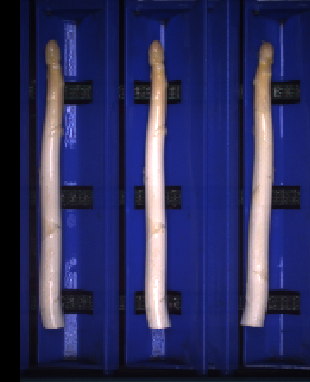
\includegraphics[width=0.9\linewidth]{Figures/appendix/violet_falsepositive_02.png}
		\vspace{-5pt}
		\caption{False Positive}
	\end{subfigure}
	\begin{subfigure}{0.3\textwidth}
		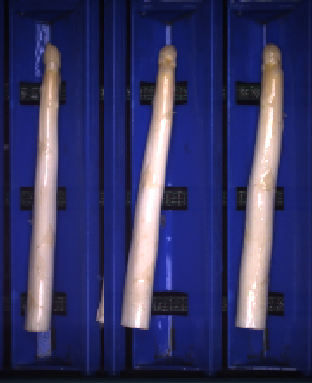
\includegraphics[width=0.9\linewidth]{Figures/appendix/violet_falsepositive_03.png}
		\vspace{-5pt}
		\caption{False Positive}
	\end{subfigure}
	\vspace{-5pt}
    \caption[Single-Label CNN Example Images Feature Violet]{\textbf{Feature Violet}~~~Randomly chosen example images of false negatives and false positives of the feature violet after 5160 training steps. In the following, suggestions for the wrong classification are given which apply only to the depicted images. The false negative examples are all cases where the presence of feature violet is only slightly remarkable, with most prominence in sample (A). Looking closer at the false positives, the asparagus in image (D) and (E) might also be slightly rose around the upper part. In image (F), the dark color at the asparagus head is probably rust. The presence and absence of feature violet might have been difficult in cases where the feature was not clearly recognizable as violet but more of a pale rose color.}
    \label{fig:ExampleImagesViolet}
\end{figure}

\begin{figure}[h]
	\centering
	\begin{subfigure}{0.3\textwidth}
		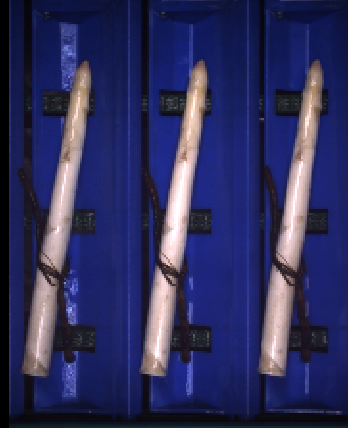
\includegraphics[width=0.9\linewidth]{Figures/appendix/fractured_falsenegative_01.png}
		\vspace{-5pt}
		\caption{False Negative}
	\end{subfigure}
	\begin{subfigure}{0.3\textwidth}
		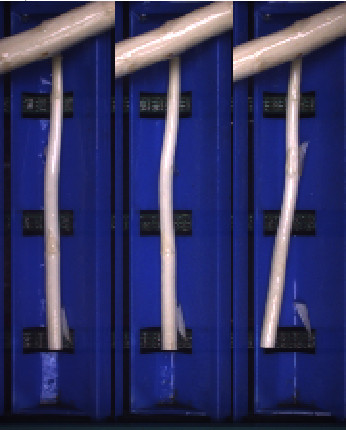
\includegraphics[width=0.9\linewidth]{Figures/appendix/fractured_falsenegative_02.png}
		\vspace{-5pt}
		\caption{False Negative}
	\end{subfigure}
	\begin{subfigure}{0.3\textwidth}
		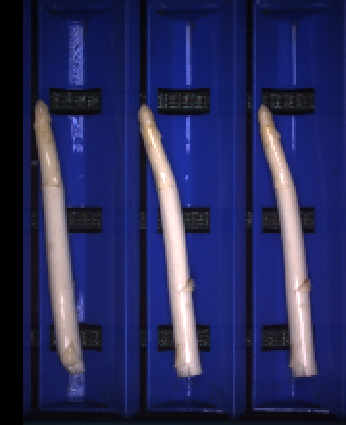
\includegraphics[width=0.9\linewidth]{Figures/appendix/fractured_falsenegative_03.png}
		\vspace{-5pt}
		\caption{False Negative}
	\end{subfigure}

	\begin{subfigure}{0.3\textwidth}
		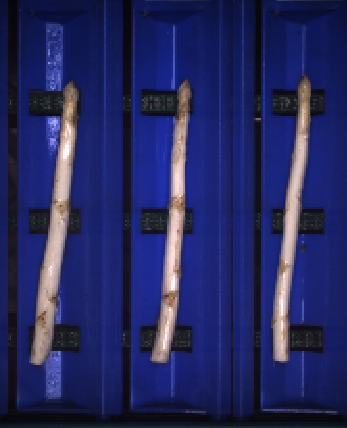
\includegraphics[width=0.9\linewidth]{Figures/appendix/fractured_falsepositive_01.png}
		\vspace{-5pt}
		\caption{False Positive}
	\end{subfigure}
	\begin{subfigure}{0.3\textwidth}
		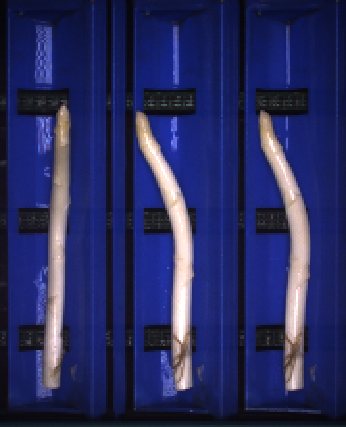
\includegraphics[width=0.9\linewidth]{Figures/appendix/fractured_falsepositive_02.png}
		\vspace{-5pt}
		\caption{False Positive}
	\end{subfigure}
	\begin{subfigure}{0.3\textwidth}
		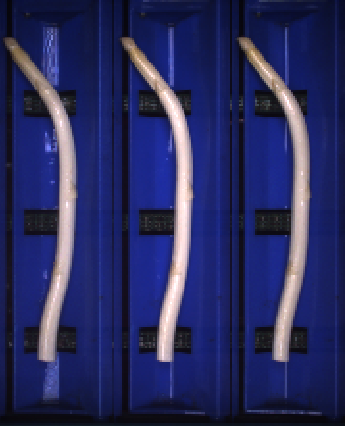
\includegraphics[width=0.9\linewidth]{Figures/appendix/fractured_falsepositive_03.png}
		\vspace{-5pt}
		\caption{False Positive}
	\end{subfigure}
	\vspace{-5pt}
	\caption[Single-Label CNN Example Images Feature Fractured]{\textbf{Single-Label CNN Example Images Feature Fractured}~~~Example images of false negatives and false positives of the feature fractured after 2700 training steps.}
	\vspace{-20pt}
    \label{fig:ExampleImagesFractured}
\end{figure}

\begin{figure}[h]
	\centering
	\begin{subfigure}{0.3\textwidth}
		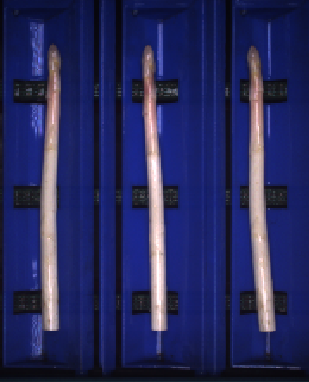
\includegraphics[width=0.9\linewidth]{Figures/appendix/flower_falsenegative_01.png}
		\vspace{-5pt} 
		\caption{False Negative}
	\end{subfigure}
	\begin{subfigure}{0.3\textwidth}
		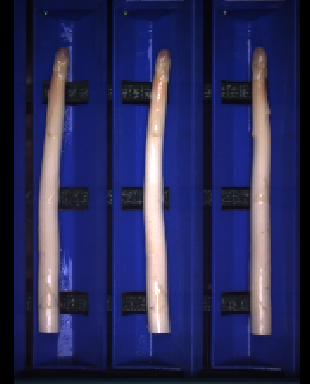
\includegraphics[width=0.9\linewidth]{Figures/appendix/flower_falsenegative_02.png}
		\vspace{-5pt}
		\caption{False Negative}
	\end{subfigure}
	\begin{subfigure}{0.3\textwidth}
		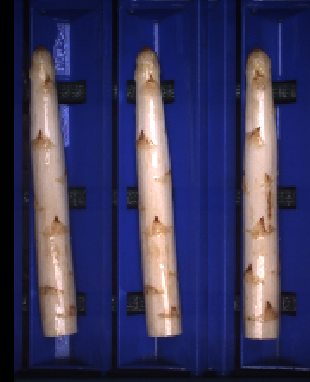
\includegraphics[width=0.9\linewidth]{Figures/appendix/flower_falsenegative_03.png}
		\vspace{-5pt}
		\caption{False Negative}
	\end{subfigure}

	\begin{subfigure}{0.3\textwidth}
		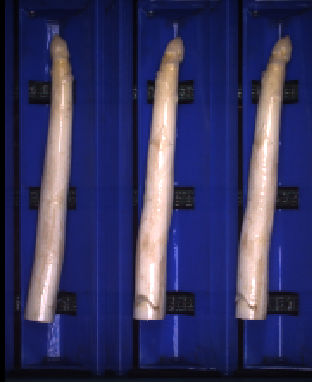
\includegraphics[width=0.9\linewidth]{Figures/appendix/flower_falsepositive_01.png}
		\vspace{-5pt} 
		\caption{False Positive}
	\end{subfigure}
	\begin{subfigure}{0.3\textwidth}
		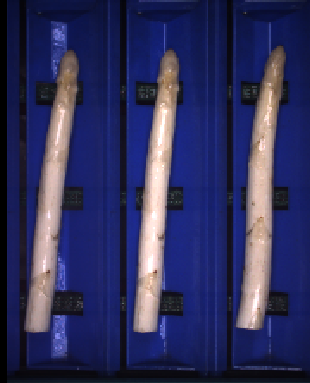
\includegraphics[width=0.9\linewidth]{Figures/appendix/flower_falsepositive_02.png}
		\vspace{-5pt}
		\caption{False Positive}
	\end{subfigure}
	\begin{subfigure}{0.3\textwidth}
		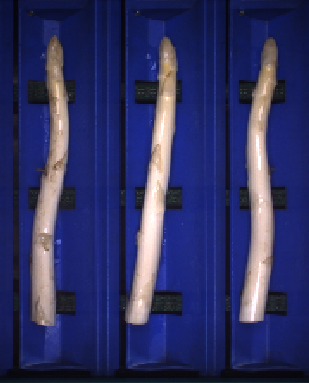
\includegraphics[width=0.9\linewidth]{Figures/appendix/flower_falsepositive_03.png}
		\vspace{-5pt}
		\caption{False Positive}
	\end{subfigure}
	\vspace{-5pt}
	\caption[Single-Label CNN Example Images Feature Flower]{\textbf{Single-Label CNN Example Images Feature Flower}~~~Example images of false negatives and false positives of the feature flower after 4800 training steps.}
		\vspace{-20pt}
    \label{fig:ExampleImagesFlower}
\end{figure}

\begin{figure}[h]
	\centering
	\begin{subfigure}{0.3\textwidth}
		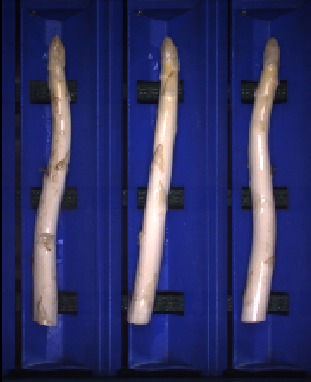
\includegraphics[width=0.9\linewidth]{Figures/appendix/rustyhead_falsenegative_01.png}
		\vspace{-5pt}
		\caption{False Negative}
	\end{subfigure}
	\begin{subfigure}{0.3\textwidth}
		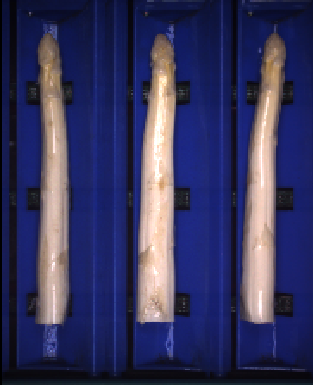
\includegraphics[width=0.9\linewidth]{Figures/appendix/rustyhead_falsenegative_02.png}
		\vspace{-5pt}
		\caption{False Negative}
	\end{subfigure}
	\begin{subfigure}{0.3\textwidth}
		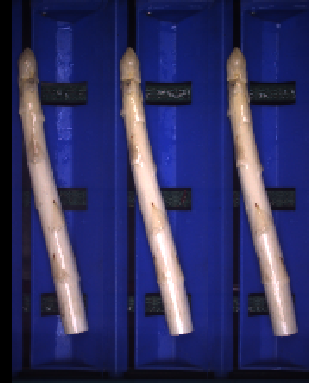
\includegraphics[width=0.9\linewidth]{Figures/appendix/rustyhead_falsenegative_03.png}
		\vspace{-5pt}
		\caption{False Negative}
	\end{subfigure}

	\begin{subfigure}{0.3\textwidth}
		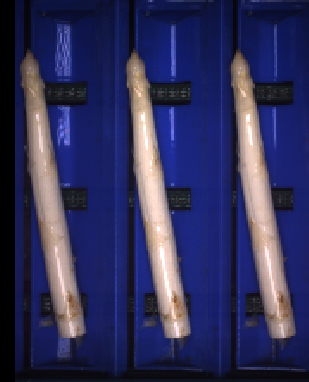
\includegraphics[width=0.9\linewidth]{Figures/appendix/rustyhead_falsepositive_01.png}
		\vspace{-5pt}
		\caption{False Positive}
	\end{subfigure}
	\begin{subfigure}{0.3\textwidth}
		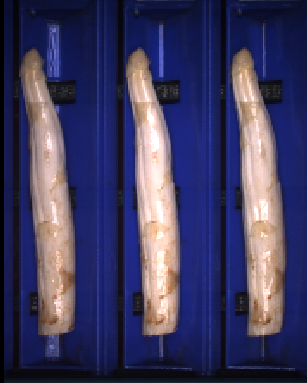
\includegraphics[width=0.9\linewidth]{Figures/appendix/rustyhead_falsepositive_02.png}
		\vspace{-5pt}
		\caption{False Positive}
	\end{subfigure}
	\begin{subfigure}{0.3\textwidth}
		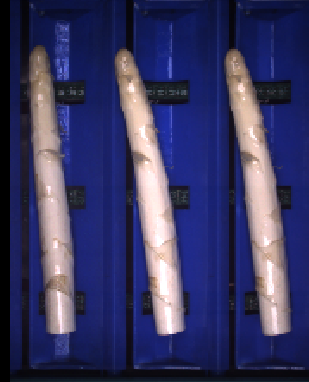
\includegraphics[width=0.9\linewidth]{Figures/appendix/rustyhead_falsepositive_03.png}
		\vspace{-5pt}
		\caption{False Positive}
	\end{subfigure}
	\vspace{-5pt}
	\caption[Single-Label CNN Example Images Feature Rusty Head]{\textbf{Single-Label CNN Example Images Feature Rusty Head}~~~Example images of false negatives and false positives of the feature rusty head after 4680 training steps.}
	\vspace{-20pt}
    \label{fig:ExampleImagesRustyHead}
\end{figure}

\begin{figure}[h]
	\centering
	\begin{subfigure}{0.3\textwidth}
		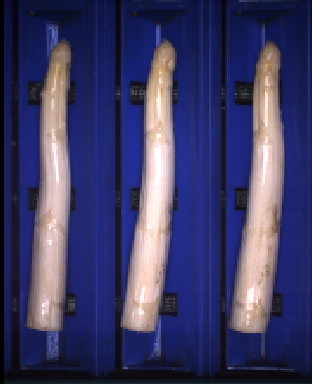
\includegraphics[width=0.9\linewidth]{Figures/appendix/rustybody_falsenegative_01.png}
		\vspace{-5pt}
		\caption{False Negative}
	\end{subfigure}
	\begin{subfigure}{0.3\textwidth}
		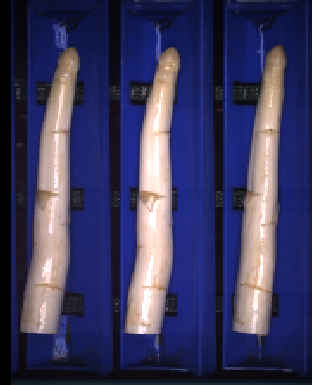
\includegraphics[width=0.9\linewidth]{Figures/appendix/rustybody_falsenegative_02.png}
		\vspace{-5pt}
		\caption{False Negative}
	\end{subfigure}
	\begin{subfigure}{0.3\textwidth}
		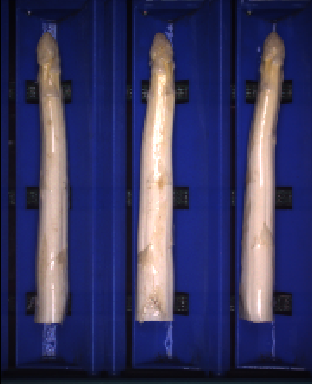
\includegraphics[width=0.9\linewidth]{Figures/appendix/rustybody_falsenegative_03.png}
		\vspace{-5pt}
		\caption{False Negative}
	\end{subfigure}

	\begin{subfigure}{0.3\textwidth}
		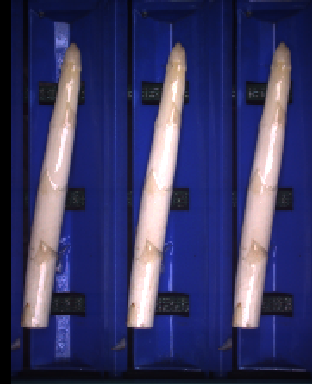
\includegraphics[width=0.9\linewidth]{Figures/appendix/rustybody_falsepositive_01.png}
		\vspace{-5pt}
		\caption{False Positive}
	\end{subfigure}
	\begin{subfigure}{0.3\textwidth}
		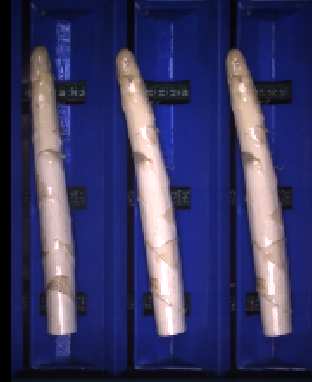
\includegraphics[width=0.9\linewidth]{Figures/appendix/rustybody_falsepositive_02.png}
		\vspace{-5pt}
		\caption{False Positive}
	\end{subfigure}
	\begin{subfigure}{0.3\textwidth}
		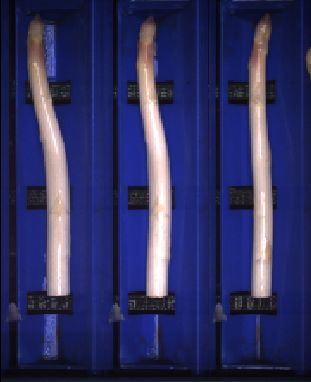
\includegraphics[width=0.9\linewidth]{Figures/appendix/rustybody_falsepositive_03.png}
		\vspace{-5pt}
		\caption{False Positive}
	\end{subfigure}
    \caption[Single-Label CNN Example Images Feature Rusty Body]{\textbf{Single-Label CNN Example Images Feature Rusty Body}~~~Example images of false negatives and false positives of the feature rusty body after 3000 training steps.}
	\vspace{-20pt}
    \label{fig:ExampleImagesRustyBody}
\end{figure}

\begin{figure}[h]
	\centering
	\begin{subfigure}{0.3\textwidth}
		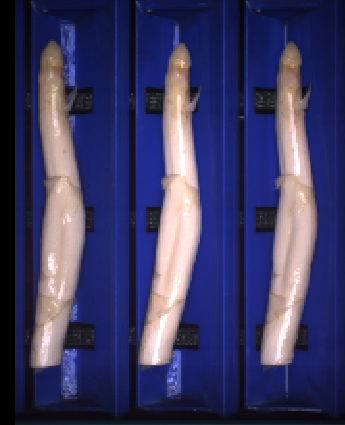
\includegraphics[width=0.9\linewidth]{Figures/appendix/verythick_falsenegative_01.png}
		\vspace{-5pt}
		\caption{False Negative}
	\end{subfigure}

	\begin{subfigure}{0.3\textwidth}
		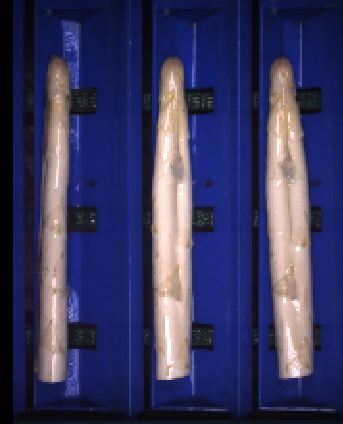
\includegraphics[width=0.9\linewidth]{Figures/appendix/verythick_falsepositive_01.png}
		\vspace{-5pt}
		\caption{False Positive}
	\end{subfigure}
	\begin{subfigure}{0.3\textwidth}
		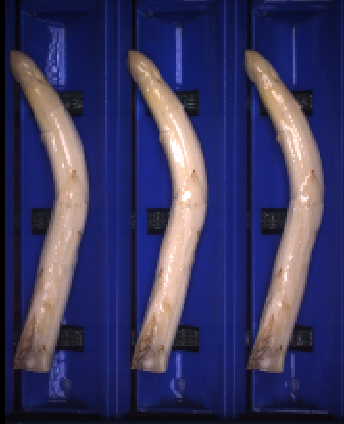
\includegraphics[width=0.9\linewidth]{Figures/appendix/verythick_falsepositive_02.png}
		\vspace{-5pt}
		\caption{False Positive}
	\end{subfigure}
	\begin{subfigure}{0.3\textwidth}
		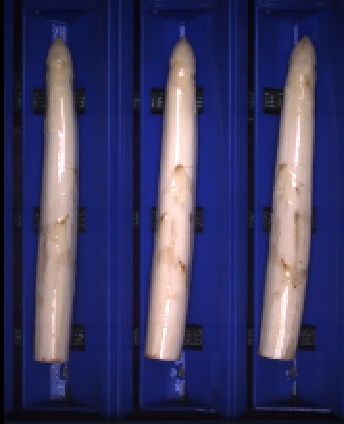
\includegraphics[width=0.9\linewidth]{Figures/appendix/verythick_falsepositive_03.png}
		\vspace{-5pt}
		\caption{False Positive}
	\end{subfigure}
    \caption[Single-Label CNN Example Images Feature Very Thick]{\textbf{Single-Label CNN Example Images Feature Very Thick}~~~Example images of false negatives and false positives of the feature very thick after 5400 training steps.}
    	\vspace{-20pt}
    \label{fig:ExampleImagesVeryThick}
\end{figure}

\begin{figure}[h]
	\centering
	\begin{subfigure}{0.3\textwidth}
		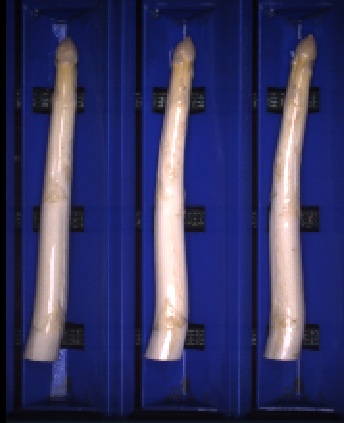
\includegraphics[width=0.9\linewidth]{Figures/appendix/thick_falsenegative_01.png}
		\vspace{-5pt} 
		\caption{False Negative}
	\end{subfigure}
	\begin{subfigure}{0.3\textwidth}
		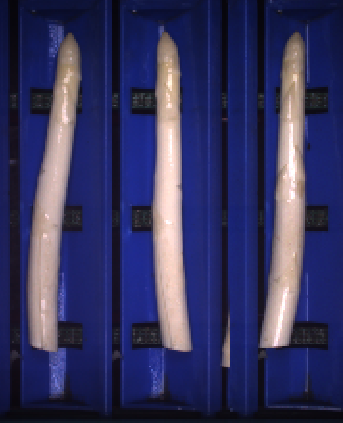
\includegraphics[width=0.9\linewidth]{Figures/appendix/thick_falsenegative_02.png}
		\vspace{-5pt}
		\caption{False Negative}
	\end{subfigure}
	\begin{subfigure}{0.3\textwidth}
		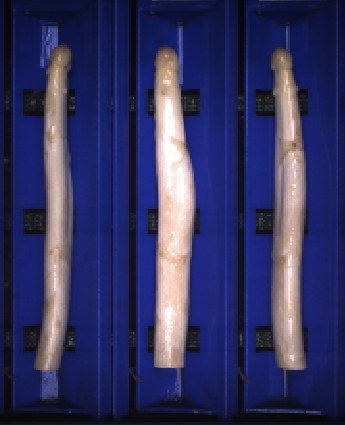
\includegraphics[width=0.9\linewidth]{Figures/appendix/thick_falsenegative_03.png}
		\vspace{-5pt}
		\caption{False Negative}
	\end{subfigure}

	\begin{subfigure}{0.3\textwidth}
		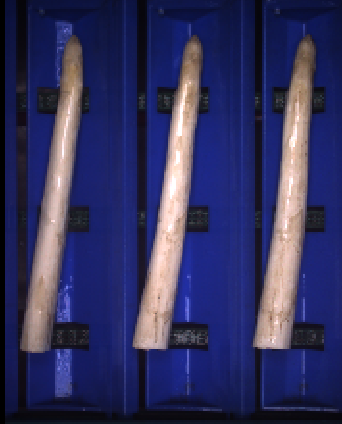
\includegraphics[width=0.9\linewidth]{Figures/appendix/thick_falsepositive_01.png} 
		\vspace{-5pt}
		\caption{False Positive}
	\end{subfigure}
	\begin{subfigure}{0.3\textwidth}
		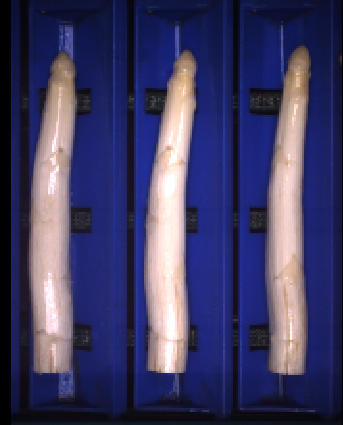
\includegraphics[width=0.9\linewidth]{Figures/appendix/thick_falsepositive_02.png}
		\vspace{-5pt}
		\caption{False Positive}
	\end{subfigure}
	\begin{subfigure}{0.3\textwidth}
		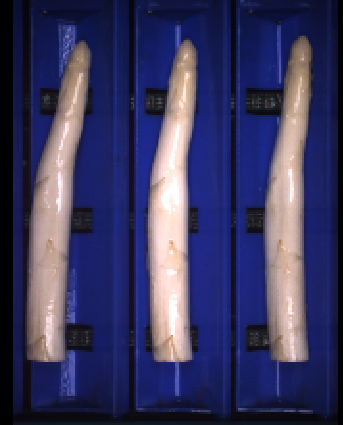
\includegraphics[width=0.9\linewidth]{Figures/appendix/thick_falsepositive_03.png}
		\vspace{-5pt}
		\caption{False Positive}
	\end{subfigure}
    \caption[Single-Label CNN Example Images Feature Thick]{\textbf{Single-Label CNN Example Images Feature Thick}~~~Example images of false negatives and false positives of the feature thick after 3960 training steps.}
	\vspace{-20pt}
    \label{fig:ExampleImagesThick}
\end{figure}

\begin{figure}[h]
	\centering
	\begin{subfigure}{0.3\textwidth}
		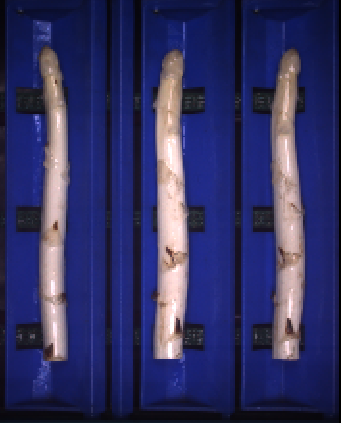
\includegraphics[width=0.9\linewidth]{Figures/appendix/medium_falsenegative_01.png}
		\vspace{-5pt} 
		\caption{False Negative}
	\end{subfigure}
	\begin{subfigure}{0.3\textwidth}
		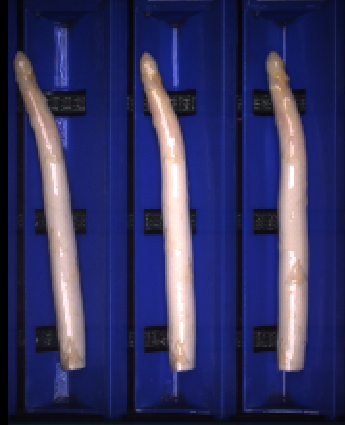
\includegraphics[width=0.9\linewidth]{Figures/appendix/medium_falsenegative_02.png}
		\vspace{-5pt}
		\caption{False Negative}
	\end{subfigure}
	\begin{subfigure}{0.3\textwidth}
		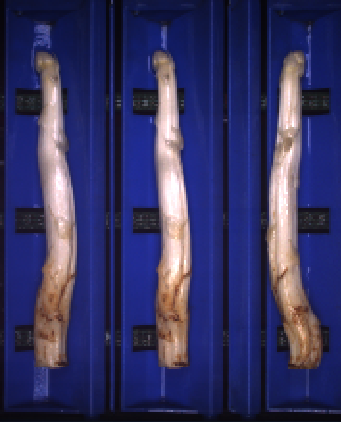
\includegraphics[width=0.9\linewidth]{Figures/appendix/medium_falsenegative_03.png}
		\vspace{-5pt}
		\caption{False Negative}
	\end{subfigure}

	\begin{subfigure}{0.3\textwidth}
		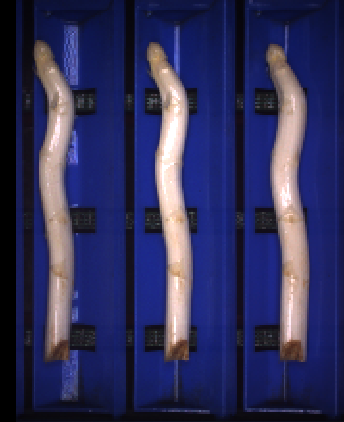
\includegraphics[width=0.9\linewidth]{Figures/appendix/medium_falsepositive_01.png}
		\vspace{-5pt} 
		\caption{False Positive}
	\end{subfigure}
	\begin{subfigure}{0.3\textwidth}
		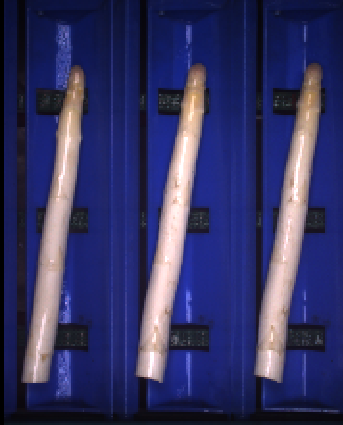
\includegraphics[width=0.9\linewidth]{Figures/appendix/medium_falsepositive_02.png}
		\vspace{-5pt}
		\caption{False Positive}
	\end{subfigure}
	\begin{subfigure}{0.3\textwidth}
		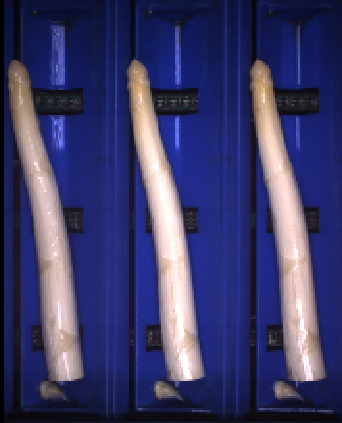
\includegraphics[width=0.9\linewidth]{Figures/appendix/medium_falsepositive_03.png}
		\vspace{-5pt}
		\caption{False Positive}
	\end{subfigure}
	\caption[Single-Label CNN Example Images Feature Medium Thick]{\textbf{Single-Label CNN Example Images Feature Medium Thick}~~~Example images of false negatives and false positives of the feature medium thick after 4560 training steps.}
	\vspace{-20pt}
    \label{fig:ExampleImagesMediumThick}
\end{figure}

\begin{figure}[h]
	\centering
	\begin{subfigure}{0.3\textwidth}
		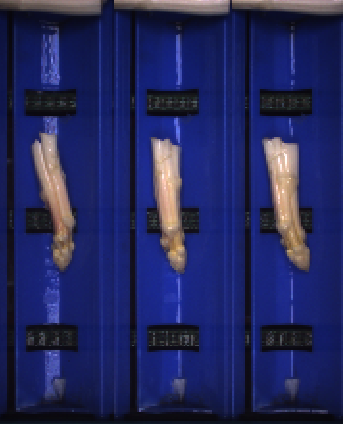
\includegraphics[width=0.9\linewidth]{Figures/appendix/thin_falsenegative_01.png} 
		\vspace{-5pt}
		\caption{False Negative}
	\end{subfigure}
	\begin{subfigure}{0.3\textwidth}
		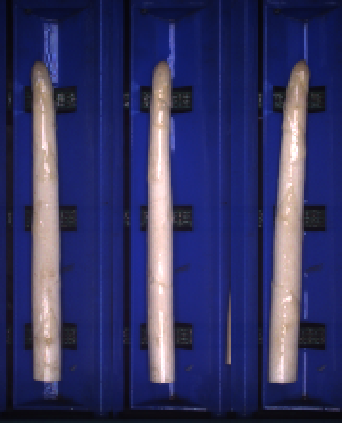
\includegraphics[width=0.9\linewidth]{Figures/appendix/thin_falsenegative_02.png}
		\vspace{-5pt}
		\caption{False Negative}
	\end{subfigure}
	\begin{subfigure}{0.3\textwidth}
		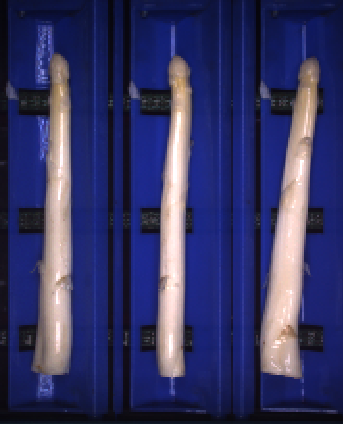
\includegraphics[width=0.9\linewidth]{Figures/appendix/thin_falsenegative_03.png}
		\vspace{-5pt}
		\caption{False Negative}
	\end{subfigure}

	\begin{subfigure}{0.3\textwidth}
		\includegraphics[width=0.9\linewidth]{Figures/appendix/thin_falsepositive_01.png}
		\vspace{-5pt} 
		\caption{False Positive}
	\end{subfigure}
	\begin{subfigure}{0.3\textwidth}
		\includegraphics[width=0.9\linewidth]{Figures/appendix/thin_falsepositive_02.png}
		\vspace{-5pt}
		\caption{False Positive}
	\end{subfigure}
	\begin{subfigure}{0.3\textwidth}
		\includegraphics[width=0.9\linewidth]{Figures/appendix/thin_falsepositive_03.png}
		\vspace{-5pt}
		\caption{False Positive}
	\end{subfigure}
	\caption[Single-Label CNN Example Images Feature Thin]{\textbf{Single-Label CNN Example Images Feature Thin}~~~Example images of false negatives and false positives of the feature thin after 4200 training steps.}
	\vspace{-20pt}
    \label{fig:ExampleImagesThin}
\end{figure}

\begin{figure}[h]
	\centering
	\begin{subfigure}{0.3\textwidth}
		\includegraphics[width=0.9\linewidth]{Figures/appendix/verythin_falsenegative_01.png}
		\vspace{-5pt} 
		\caption{False Negative}
	\end{subfigure}
	\begin{subfigure}{0.3\textwidth}
		\includegraphics[width=0.9\linewidth]{Figures/appendix/verythin_falsenegative_02.png}
		\vspace{-5pt}
		\caption{False Negative}
	\end{subfigure}
	\begin{subfigure}{0.3\textwidth}
		\includegraphics[width=0.9\linewidth]{Figures/appendix/verythin_falsenegative_03.png}
		\vspace{-5pt}
		\caption{False Negative}
	\end{subfigure}

	\begin{subfigure}{0.3\textwidth}
		\includegraphics[width=0.9\linewidth]{Figures/appendix/verythin_falsepositive_01.png}
		\vspace{-5pt}
		\caption{False Positive}
	\end{subfigure}
	\begin{subfigure}{0.3\textwidth}
		\includegraphics[width=0.9\linewidth]{Figures/appendix/verythin_falsepositive_02.png}
		\vspace{-5pt}
		\caption{False Positive}
	\end{subfigure}
	\begin{subfigure}{0.3\textwidth}
		\includegraphics[width=0.9\linewidth]{Figures/appendix/verythin_falsepositive_03.png}
		\vspace{-5pt}
		\caption{False Positive}
	\end{subfigure}
	\caption[Single-Label CNN Example Images Feature Very Thin]{\textbf{Single-Label CNN Example Images Feature Very Thin}~~~Example images of false negatives and false positives of the feature very thin after 4320 training steps.}
	\vspace{-20pt}
    \label{fig:ExampleImagesVeryThin}
\end{figure}

\begin{figure}[h]
	\centering
	\begin{subfigure}{0.3\textwidth}
		\includegraphics[width=0.9\linewidth]{Figures/appendix/notclassifiable_falsenegative_01.png}
		\vspace{-5pt}
		\caption{False Negative}
	\end{subfigure}
	\begin{subfigure}{0.3\textwidth}
		\includegraphics[width=0.9\linewidth]{Figures/appendix/notclassifiable_falsenegative_02.png}
		\vspace{-5pt}
		\caption{False Negative}
	\end{subfigure}
	\begin{subfigure}{0.3\textwidth}
		\includegraphics[width=0.9\linewidth]{Figures/appendix/notclassifiable_falsenegative_03.png}
		\vspace{-5pt}
		\caption{False Negative}
	\end{subfigure}

	\begin{subfigure}{0.3\textwidth}
		\includegraphics[width=0.9\linewidth]{Figures/appendix/notclassifiable_falsepositive_01.png}
		\vspace{-5pt} 
		\caption{False Positive}
	\end{subfigure}
	\begin{subfigure}{0.3\textwidth}
		\includegraphics[width=0.9\linewidth]{Figures/appendix/notclassifiable_falsepositive_02.png}
		\vspace{-5pt}
		\caption{False Positive}
	\end{subfigure}
	\begin{subfigure}{0.3\textwidth}
		\includegraphics[width=0.9\linewidth]{Figures/appendix/notclassifiable_falsepositive_03.png}
		\vspace{-5pt}
		\caption{False Positive}
	\end{subfigure}
    \caption[Single-Label CNN Example Images Feature Not Classifiable]{\textbf{Single-Label CNN Example Images Feature Not Classifiable}~~~Example images of false negatives and false positives of the feature not classifiable after 5400 training steps.}
	\vspace{-20pt}
    \label{fig:ExampleImagesNotClassifiable}
\end{figure}

\begin{figure}[!htb]
	\centering
	\begin{subfigure}{0.49\textwidth}
		\includegraphics[width=\linewidth]{Figures/appendix/fractured_test_accuracy.png} 
	\end{subfigure}
	\begin{subfigure}{0.49\textwidth}
		\includegraphics[width=\linewidth]{Figures/appendix/fractured_test_loss.png}
	\end{subfigure}

	\begin{subfigure}{0.49\textwidth}
		\includegraphics[width=\linewidth]{Figures/appendix/fractured_train_accuracy.png} 
	\end{subfigure}
	\begin{subfigure}{0.49\textwidth}
		\includegraphics[width=\linewidth]{Figures/appendix/fractured_train_loss.png}
	\end{subfigure}
    \caption[Single-Label CNN Accuracy and Loss]{\textbf{Accuracy and Loss of Feature Fractured}~~~Test accuracy and test loss as well as training accuracy and training loss for the feature fractured are depicted above. It was randomly chosen to show an exemplary course of accuracy and loss during training.}
    \label{fig:ExamplePlotsFractured}
\end{figure}